% =============================================================================
% Chapter 4 — Findings: The Systematic Map
% =============================================================================

\chapter{Findings: The Systematic Map}
\label{ch:findings}

\section{The Shape of the Corpus}
\label{sec:shape}

The final corpus comprises 275 records: 151 identified through database searches (Web of Science, Scopus, Policy Commons) and 124 through backward and forward citation chaining on four anchor texts (Graham 2006; Weizman 2007; Kitchin 2014; Michael 2007). Full extraction and coding succeeded for 270 records (98.2\%); the five failures — three unretrievable PDFs, one wrong-source document, one record without full text — are documented in Section~\ref{sec:limitations}.

Three structural features of the corpus matter for what follows.

First, \textit{recency}. The literature is overwhelmingly a twenty-first-century phenomenon, and predominantly a post-2010 one: 111 records date from the 2010s and 136 from the 2020s alone, against 16 from the 2000s. Publication peaks in 2024 (n=28). The convergence this dissertation examines — algorithmic governance meeting urban destruction — is being theorised now, in real time, and a substantial fraction of the destruction-side literature concerns events still unfolding at the time of writing.

Second, \textit{genre}. Journal articles dominate (69\%), but the corpus is notably hybrid: book chapters (11\%), conference papers (8\%), and policy reports and grey literature (7\%) each carry distinct epistemic weight. The grey literature is not filler. The UK Ministry of Defence's Future Cities reports, the US-China Economic and Security Review Commission's analysis of Chinese smart-city development, and NATO-adjacent technical papers on military exploitation of smart-city IoT constitute a practitioner literature that confirms, from inside the defence establishment, the feasibility claims the critical literature makes from outside (Section~\ref{sec:theme1}).

Third, \textit{method}. The corpus skews interpretive: theoretical work (34\%) and qualitative empirical work (23\%) dominate, with case studies at 15\% and policy analysis at 10\%. Quantitative empirical work is scarce (7\%). This is itself a finding: the intersection of algorithmic governance and spatial destruction has been theorised and narrated far more than it has been measured — with the striking exception of remote-sensing damage assessments of Gaza \parencite{holail2024}, where the same sensing stack used for targeting is turned to documentation.

\begin{table}[H]
\centering
\caption{Mean theme scores by corpus (0–3 scale; n scoring $\geq$2 in parentheses)}
\label{tab:themes}
\begin{tabular}{lcccc}
\toprule
\textbf{Theme} & \textbf{Search A (n=147)} & \textbf{Snowball (n=123)} & \textbf{Combined (n=270)} \\
\midrule
T1: Dual-Use Fluidity & 1.21 (48) & 0.92 (38) & 1.08 (86) \\
T2: Epistemic Authority & 1.43 (72) & 0.98 (45) & 1.22 (117) \\
T3: Machinic City & 1.31 (65) & 0.84 (37) & 1.10 (102) \\
T4: Spatial Destruction & 0.32 (18) & 1.81 (58) & 0.98 (76) \\
\bottomrule
\end{tabular}
\end{table}

The asymmetry in Table~\ref{tab:themes} is the corpus's first lesson. The keyword-search corpus and the citation-network corpus are not two samples of one literature; they are two literatures that barely cite each other. Database searching recovered the governance side — dual-use transfer, epistemic authority, the programmable city. Citation chaining from Graham and Weizman recovered the destruction side — urbicide, domicide, home unmaking — which keyword searching had largely missed (only 18 of 147 main-corpus records score~$\geq$2 on Theme~4, against 58 of 123 snowball records). The discursive separation first visible at deduplication — zero records appearing in both searches (§\ref{sec:screening}) — is reproduced at corpus scale. Michael (2007), notably, yielded no included records at all: the epistemic-authority literature it anchors was already captured by the Weizman and Graham networks, and the counterinsurgency-theory branch does not intersect the urban-analytics branch. The literatures of how algorithms govern and how cities are destroyed run in parallel. Mapping where they meet is the task of this chapter.

\begin{figure}[H]
\centering
\makebox[\textwidth][c]{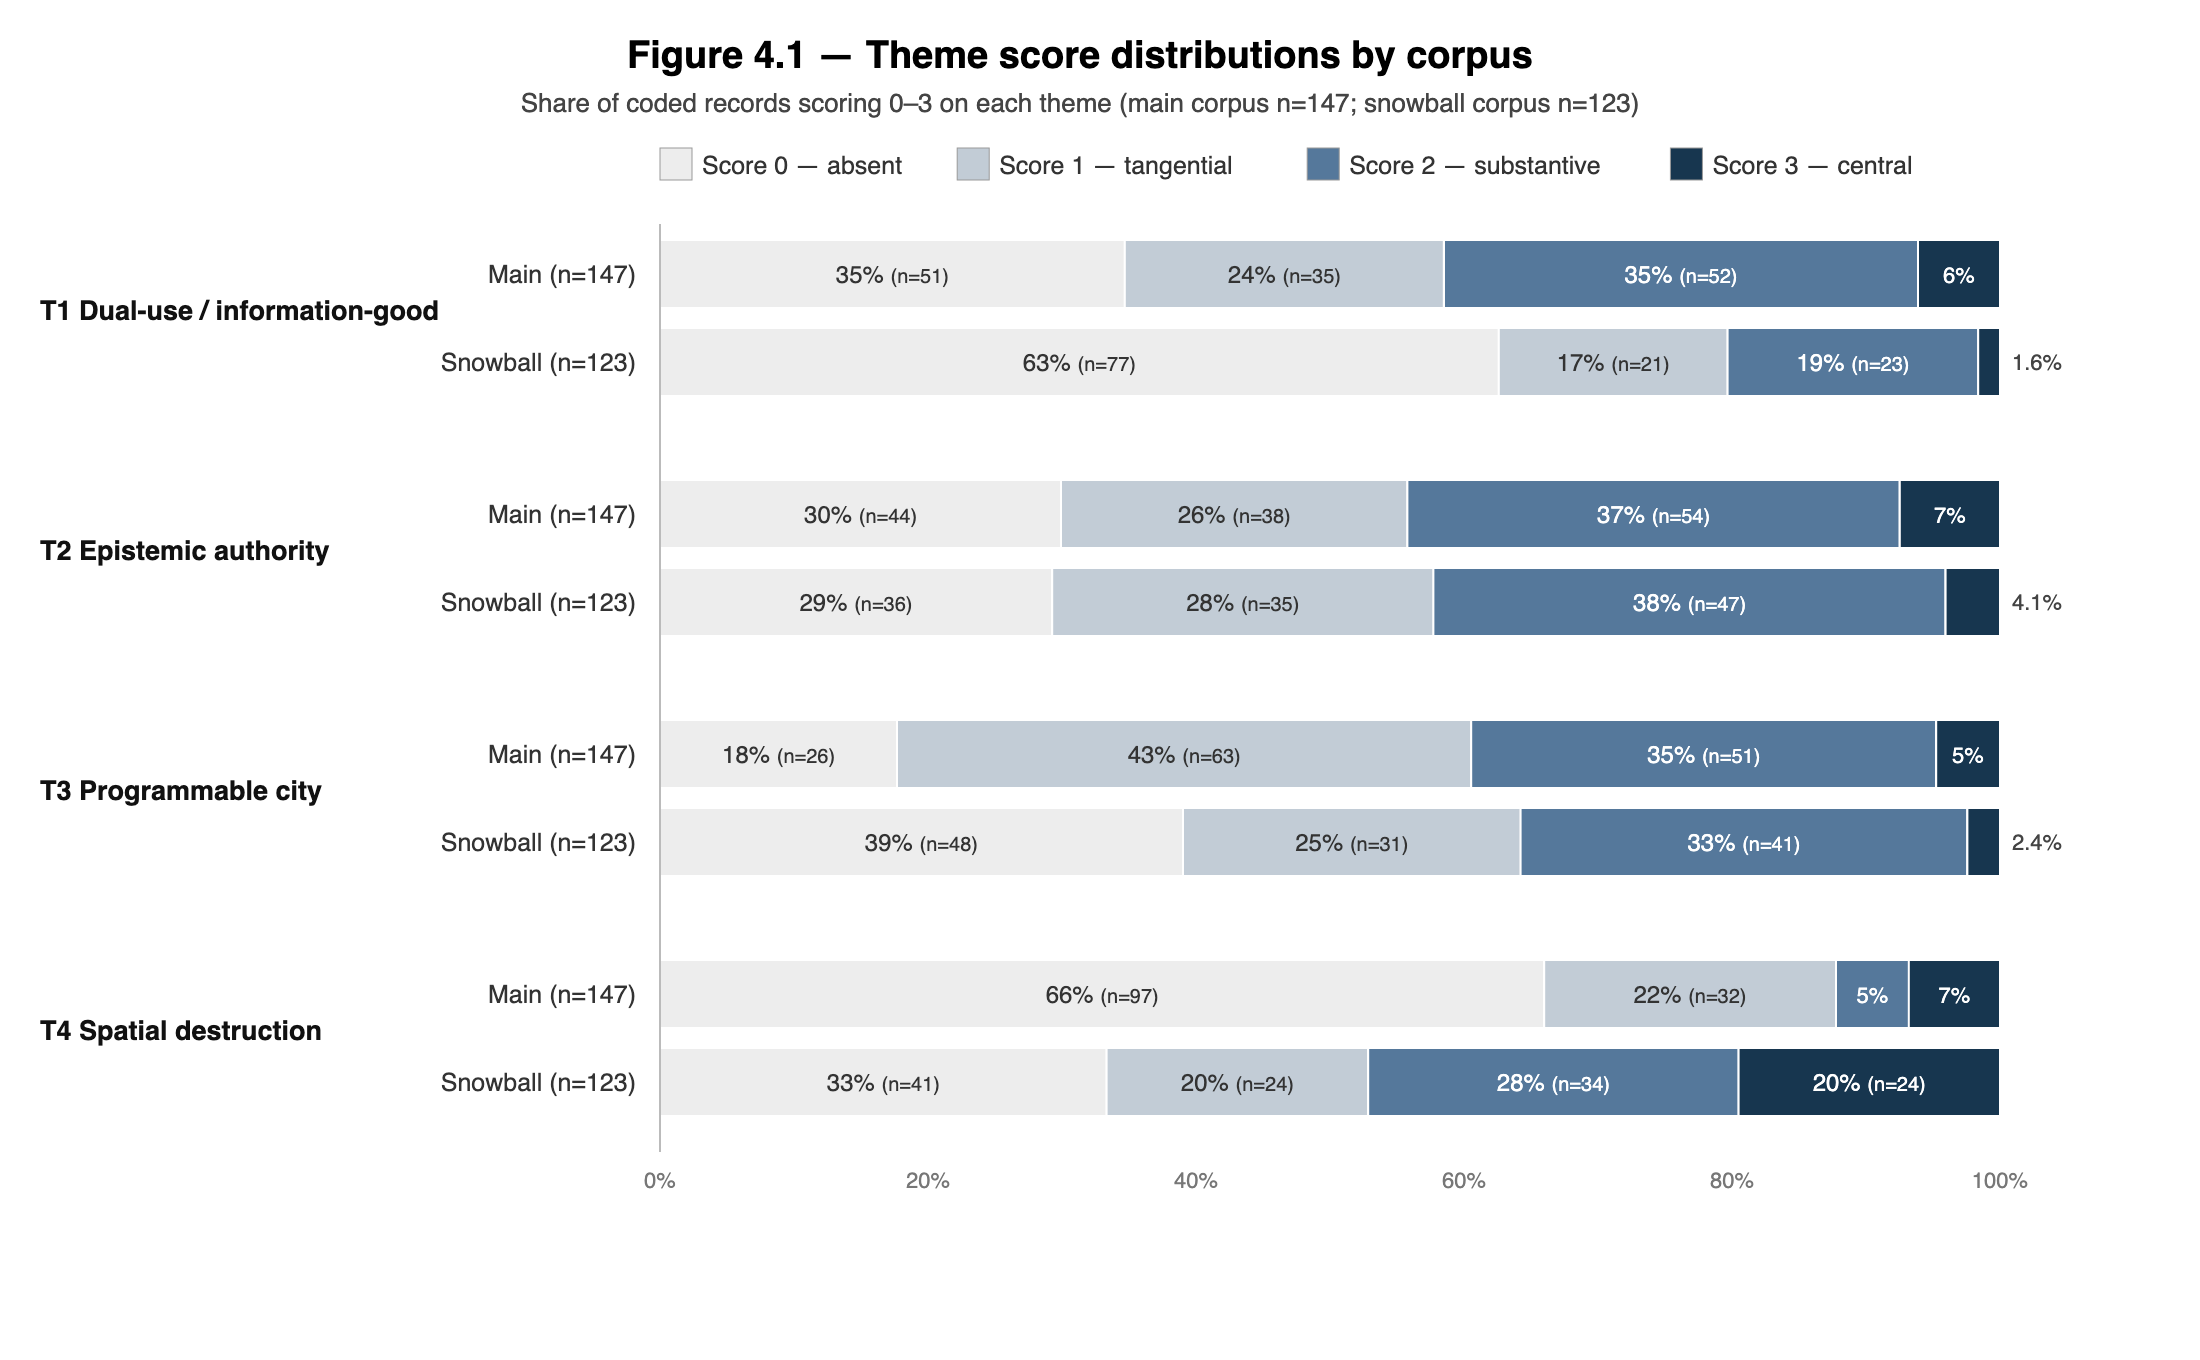
\includegraphics[width=1.16\textwidth]{figures/figure_4_1_theme_distributions.png}}
\caption{Theme score distributions by corpus (share of coded records)}
\label{fig:themes-dist}
\end{figure}

\section{Theme 1 — The Dual-Use Mechanism ($n=86$ scoring $\geq$2)}
\label{sec:theme1}

The first theme asked whether the literature treats algorithmic and urban-analytic systems as dual-use: transferable between civilian governance and military application with minimal modification. The answer is an emphatic yes — but with a structure, and a hole.

\subsection{Dual-use as design goal: the practitioner literature}

The largest cluster ($\sim$18 records) is one this dissertation did not expect to find in such volume: technical and defence-planning literatures that affirmatively engineer the military exploitation of civilian smart-city infrastructure. A series of NATO-adjacent papers proposes architectures for integrating smart-city IoT into military information systems — mapping urban sensor data onto NATO data models for ``situational awareness'' in urban operations (Pradhan et al., 2018; Riberto et al., 2018; Johnsen et al., 2018; Suri et al., 2018). \textcite{tsiolis2025} make the logic explicit in their title: an ``Internet of Military Defense Things'' that assumes ``future military forces will have to conduct a range of operations'' inside ``permissive intelligent urban operational environments.'' The UK DCDC Future Cities reports (2019; 2020) analyse smart-city infrastructure as both opportunity and vulnerability for British forces; US Army Engineer Research and Development Center (ERDC) literature advocates ``rapid dual-use development of commercial technologies'' for force protection on domestic installations, explicitly treating the civilian smart-city technology stack as a military resource.

Two things follow. First, the transfer mechanism the framework predicts (Chapter~2) is not speculative: practitioners name it — interoperability standards (MQTT, NGVA, MIP), commercial off-the-shelf components, open data services. Second, the direction of transfer in this cluster is overwhelmingly civilian-to-military, and it is celebrated rather than lamented. The critical literature's ``boomerang'' \parencite{graham2012} here appears as a feature.

\subsection{The boomerang: war-zone technology comes home}

The mirror cluster ($\sim$16 records) is the critical canon on military-to-civilian transfer. \textcite{wiig2018} traces counterinsurgency tactics and technologies from Iraq and Afghanistan into the Camden Metro Police Department. \textcite[p.~4]{wall2013} names the ``green-to-blue pipeline'' by which military drones become domestic policing tools, and explicitly theorises ``dual-use scopic technologies'' (p.~2). The genealogy of predictive policing runs through the Pentagon: PredPol descends from Army Research Office funding and battlefield-casualty modelling in Iraq (Sharma \& Nijjar, 2024; The Public History and Private Future of Police Data, 2021), and Palantir's software moved from counterinsurgency to the LAPD (Predict and Surveil, 2021). \textcite{coaffee2015} documents ANPR cameras ``developed from former military technology'' redeployed across British civic space; \textcite{kitchin2014} tracks the Long-Range Acoustic Device (LRAD) — a non-lethal directed-energy weapon developed for maritime force protection — from Somali pirate deterrence to crowd control at the Toronto G20. \textcite{schimmel2021} extends the boomerang logic into the domain of spectacle: the NFL's security infrastructure is legally classified alongside Pentagon suppliers under the SAFETY Act, and stadiums are operationalised as domestic security laboratories — crowd-monitoring technologies tested on football fans migrate to policing contexts. Schimmel's analysis demonstrates that the civil–military dual-use circuit is not limited to overtly ``security'' domains but operates wherever large populations are gathered, tracked, and managed.

\subsection{Commercial data, state security}

A third cluster ($\sim$12 records) documents the flow of commercially generated data into security apparatus — the surveillance-capitalism/state nexus. \textcite{amoore2009} provides the corpus's most developed account: association-rule algorithms honed on Marks \& Spencer and Wal-Mart customer data reappear in US VISIT and e-borders, security practices ``oscillating'' between commercial and military spheres. \textcite{wilhelmsen2022} shows commercial location data repurposed for espionage; Our Incriminating Lives (2023) documents Palantir fusing utility bills, foreclosure records, and LexisNexis into LAPD dragnets; Big Brother Watch (2019) traces Experian's Mosaic marketing segments into Durham Constabulary's Harm Assessment Risk Tool (HART) for recidivism prediction.

\subsection{Dual-use as geostrategy}

A fourth cluster ($\sim$8 records) treats dual-use as state strategy: China's ``safe city'' exports as vehicles of civil-military fusion and geopolitical influence \parencite{weber2023} — the urban ``city brain'' whose architecture derives from, and feeds, military command brains \parencite{atha2020,robinson2020} — with parallel dynamics in Gulf smart-city procurement \parencite{ziadah2021}.

\subsection{The hole: nobody prices the transfer}

Here is the gap. Across 86 records engaging dual-use, the coders' recurring annotation — ``does not engage with the economic properties of information goods'' — appears on the large majority. The literature documents that transfer happens, richly, in both directions, across dozens of cases. It almost never asks \textit{why} it is frictionless: why software, unlike the bulldozer or the water network, moves between domains at near-zero marginal cost, carrying its ontologies with it. Only \textcite{amoore2009,wilhelmsen2022,srivastava2021} gesture at the cost structure of information goods. A distinct older literature on physical dual-use — infrastructure weaponised or sanctioned \parencite{salamanca2011,coward2009,zeitoun2018,coyles2017} — makes the contrast visible: pipes and generators can be repurposed only slowly, visibly, and at cost, and dual-use sanctions can bite (Zeitoun's Basrah, where import restrictions on ``dual-use'' parts crippled water repair). Software escapes this friction. The corpus thereby validates the dissertation's first theoretical move — Arrow's information-good economics as the missing mechanism — precisely by leaving it unmade.

\section{Theme 2 — Epistemic Authority and the Black Box ($n=117$ scoring $\geq$2)}
\label{sec:theme2}

The second theme is the corpus's most populated: how algorithmic systems acquire the authority to define truth, and how that authority is insulated from challenge. Three findings stand out.

\subsection{The pattern is political}

The predictive-policing literature ($\sim$22 records) has matured into a genuine epistemology of algorithmic governance. \textcite[p.~2]{kaufmann2019} states the core problem cleanly: patterns are ``the epistemological core of predictive policing,'' and ``the clean surface of the pattern makes it impossible to defend oneself against their results.'' Studies of specific systems show political choices being laundered into code: Rio's CrimeRadar naturalises its designers' assumptions ``in the process of translating crime events into strings of codes, datasets, and maps'' (The Making of Crime Predictions, 2021); the pattern's authority is rearticulated with each technical generation \parencite{halterlein2021}. Ethnographic work complicates the automation story from inside: Bogotá police ``corrupt'' crime data at input through institutional cultures \parencite{barreneche2019}; LAPD officers dismiss risk scores as ``witchcraft'' (Police Pushback, 2017) while nonetheless being governed by them.

\subsection{Opacity is manufactured, not inherited}

The second finding reframes the black box. Across legal and policy records ($\sim$15), opacity is not a technical property of machine learning but an institutional product: trade secrecy asserted by vendors (Predict and Surveil, 2021; Coding Inequality, 2019), procurement frameworks where ``opacity is normalised as a feature and not a bug'' (Myanmar CCTV, 2022), and statutory carve-outs that exempt national security from transparency law — the LED and AI Act ``fail to lift the `veil of secrecy''' \parencite[p.~22]{erdogan2024}, whose individualised remedies ``cannot correspond to effects of AI technologies at a population-level.'' EPIC's amicus work (2026) catches the resulting bind: automated license plate recognition (ALPR) decisions are ``cloaked in objectivity and hidden in a proprietary black box,'' making constitutional and legal oversight structurally impossible — as EPIC's Fourth Amendment framing demonstrates for the US context, and as \textcite{erdogan2024} extends to the European regulatory framework. The implication for the framework: technical transparency fixes (explainable AI, audits) recur in the corpus as necessary but radically insufficient, because the box is legal before it is computational.

\subsection{Race is constitutive, not contaminating}

The third finding is the corpus's strongest normative current ($\sim$14 records). Against the ``bias'' framing — neutral systems corrupted by skewed data — \textcite{sharma2024} argue that ``policing does not have a `racist history'. Policing makes race,'' and algorithms ``cannot `code out' race from American policing because race is an originary policing technology.'' \textcite[p.~4]{ziadah2021} documents ``digital epidermalization'' in the UAE; \textcite[p.~11]{irungbam2026} frames Manipur's internet shutdowns as ``epistemicide'' — the erasure of subaltern knowledge as a governing technique. The occupation literature extends this to epistemic sovereignty over territory: at Qalandia, ``uncertainty becomes the ultimate system of control'' \parencite[p.~8]{tawil2011}; in East Jerusalem the state manages ``the uneven distribution of visual rights'' \parencite[p.~5]{shalhoub2017}. This cluster is where Michael's \parencite{michael2007} epistemic-authority concept gets its sharpest empirical elaboration: the authority to define truth is inseparable from the authority to decide whom truth targets.

A bridging motif recurs across all three: the view from above as an epistemic position — the ``God's Eye View'' \parencite{monroe2017}, the drone's ``cosmic view'' (Wall, 2011), the helicopter's ``verticalized omniscience'' (Vertical Security, 2010), Graham's \parencite{graham2012} machinic ``Id-ing'' replacing social identification. Epistemic authority in this literature is literalised as altitude. Theme~4 shows what that altitude is for.

\section{Theme 3 — The City as Programmable System ($n=102$ scoring $\geq$2)}
\label{sec:theme3}

The third theme coded whether the literature conceptualises the city itself as a programmable, data-driven system subject to continuous modulation — the Deleuzian-De Landan ontology (Chapter~2). The answer comes from three directions that rarely cite each other.

Smart-city advocates and their critics share an ontology. Urban Operating Systems are analysed as a ``diagram of control'' that ``does not function to represent\dots\ but rather constructs a real that is to come'' \parencite[p.~7]{marvin2017}. Realtime urbanism names latency itself as a governing logic that ``naturalize[s] control as responsiveness, and collapse[s] deliberation into automation'' \parencite[p.~2]{lotfijam2025}. The smart-city critique — Kitchin's (2018) ``smartmentality,'' Tenney's (2016) ``algorithmic-regulation,'' Williamson's (2015) ``programmable environments'' — takes the same city-as-system ontology as given, contesting its politics rather than its feasibility.

Modulation runs through more channels than dashboards. A distinctive sub-current tracks control exercised through environment and affect: ``scripted architecture'' using light, smell, and sound as ``pastoral power'' \parencite[p.~7]{schuilenburg2018}; the Eindhoven nightlife living lab whose operators are ``Big Brother only to the masses'' \parencite{jacobs2024}; ``atmospheric fortification'' \parencite[p.~1]{fregonese2024}; time itself as ``an infrastructure of control'' in East Jerusalem \parencite[p.~4]{baumann2019}. The living-lab literature \parencite{jacobs2024,taylor2021} adds the city as experiment, populations enrolled as unwitting test subjects.

The military independently arrives at the same city. The hinge finding of this theme: defence doctrine converges on the identical ontology. DARPA's Combat Zones That See aimed to ``build up fully representative data profiles on the `normal' time-space movement patterns of entire subject cities so that algorithms could then use statistical modelling to `determine what is normal and what is not''' \parencite[p.~12]{graham2008}. US military urban doctrine treats the city as a ``system-of-systems,'' a ``living organism'' to be managed \parencite{danielsson2025}; China's ``city brain'' is explicitly an OODA loop \parencite{weber2023}. And a corrective to presentism runs underneath: the administered and occupied city modulated populations bureaucratically long before software — Belfast's ``controlled allocation'' of tenancies as pre-emptive spatial design \parencite[p.~9]{coyles2017}, the French colonial Section Administrative Urbaine's (SAU) remapping of Algiers ``into militarized zones'' \parencite{crane2017}, Gaza's electricity and water switched on and off as ``elastic'' humanitarian calibration \parencite[p.~1]{salamanca2011}. Algorithmic governance automates and intensifies an older administrative modulation; it does not invent it. The significance for the framework is that the programmable-city ontology is not contested between the literatures — it is shared by smart-city advocates, critical urban theorists, and military doctrine alike. What is contested is only who holds the controls.

\section{Theme 4 — Spatial Destruction and Home Unmaking ($n=76$ scoring $\geq$2)}
\label{sec:theme4}

The fourth theme is the corpus's most intense: 34 of 76 records score 3, the highest saturation of any theme. This is the literature the keyword search missed and the citation network delivered (Table~\ref{tab:themes}).

\subsection{The urbicide canon and its paradigmatic case}

The conceptual spine runs from Graham's \parencite{graham2004} ``postmortem city'' — war as ``the most thorough-going\dots\ occasion of collective violence that destroys places'' (Hewitt, cited therein) — through urbicide's tripartite definition: the killing of cosmopolitan mixing, of the means of modern urban living, and of those cast as ``unmodern'' \parencite{graham2012}. \textcite[p.~3]{hanafi2012} ``spacio-cide'' names the Palestinian variant: ``the weapons of mass destruction are not so much tanks as bulldozers.''

Palestine is the corpus's gravitational centre ($\sim$25 records), functioning explicitly as laboratory (\cite{cook2008}: confined spaces as ``laboratories where experiments to encourage Palestinian despair\dots\ are being refined''). Every modality of destruction is documented: home demolition as planning instrument \parencite{meade2011,pazfuchs2010}; ``walking through walls'' \parencite{bleibleh2015}; closure, checkpoint, and enclave \parencite[p.~10]{peteet2015} — Weisglass's ``diet, but not\dots\ die of hunger''; settlement as territorialisation \parencite{volinz2019}; sensory warfare \parencite{shalhoub2017}. \textcite[p.~1]{golanska2022} ``slow urbicide'' names the attritional register: bureaucratic neglect, pollution, obliteration of the vernacular as violence at low visibility. And the register has accelerated: \textcite[p.~3]{benguita2025} reads Gaza 2023–25 as ``Spatial Nakba'' — ``Gaza is not merely being bombed — it is being unmade as a space of collective identity and political potential'' — while Holail et al.\ \parencite{holail2024} quantify the escalation through time-series satellite sensing.

\subsection{Destruction as cycle: razing, renewal, razing}

A second cluster corrects any event-based reading. Urban renewal produces the displaceability that later warfare exploits \parencite{genc2021,coyles2017}, and post-conflict reconstruction continues the war by other means: Turkey's tabula rasa rebuilding of Sur replaces ``vernacular and communal architecture'' with housing that ``integrate[s residents] into state agencies and mortgage regimes'' \parencite[p.~16]{smith2022}; \textcite[p.~2]{hourani2024} names the ``post-conflict-catastrophe complex.'' \textcite[p.~2]{wilson2026} push the continuum furthest into peacetime, introducing ``Dracula urbanism'' to name the process by which real-estate development itself becomes a mode of slow domicide: displacement by market logic, where the violence of eviction becomes administratively routine and the smart city's optimisation mandate provides the technical language for its execution. Rio's ``Museum of Evictions'' (Arantes \& Ribeiro, 2021), Cape Town's securitised renewal \parencite{samara2010}, and the MOVE bombing's destruction of a Philadelphia block \parencite{massaro2015} extend the continuum across regime types. Domicide, the corpus insists, is a spectrum practice of states, not a wartime aberration.

\subsection{The warrant: ``dual-use'' inside the destruction}

The single most important finding for the dissertation's thesis sits here. Benguita's \parencite{benguita2025} coding of Gaza 2023–25 surfaces the exact vocabulary: ``Hospitals, schools, mosques, media institutions, and universities have been struck under the rationale of dual-use or symbolic alignment with resistance'' (emphasis added). The legal-military category of \textit{dual-use} — the same category that governs export controls and sanctions in Theme~1 — operates inside the destruction literature as the warrant for striking civilian fabric. \textcite{coward2009} documented the same logic in Iraq's ``dual use facilities''; \textcite{graham2004} recorded the USAF planner's concession that targeting dual-use electrical infrastructure killed up to 100,000 civilians. The thesis that algorithmic governance and spatial destruction share a dual-use logic is therefore not an analogy this dissertation imposes on the material: it is a connection the material states about itself.

\subsection{The thin edge: algorithmic destruction}

Yet the algorithmic mode of destruction is the theme's thinnest cluster — five records, all 2021 or later. \textcite[p.~2]{hourani2024} discusses Lavender and Where's Daddy?: AI systems generating kill lists, targets ``tracked to their homes, where they are killed along with their families,'' which ``gives lie to technophilic dreams of the sanitary smart bomb.'' \textcite{lotfijam2025} addresses AI-assisted kill chains; \textcite{zavrsnik2021} dissect Project Maven; \textcite{graham2008} reads Combat Zones That See as precursor; Holail et al.\ \parencite{holail2024} show the sensing stack's documentary afterlife. Against 76 destruction records and 117 epistemic-authority records, these five constitute the only sustained bridges. The urbicide canon theorises destruction but barely touches its algorithmisation; the algorithmic-governance literature theorises modulation but stops short of the kill chain. The intersection — algorithmically mediated urbicide — is nearly empty. This is the dissertation's central empirical finding, and it is a finding about the literature itself.

\section{The Map as Argument}
\label{sec:map-as-argument}

Read together, the four themes form the causal chain the framework predicted, and the corpus maps each link with sharply varying density:

\begin{itemize}
\item \textbf{Mechanism (T1, 86):} transfer is documented exhaustively, in both directions — but its economic grammar is untheorised.
\item \textbf{Authority (T2, 117):} the black box is shown to be institutionally manufactured, and its truths constitutively racialised.
\item \textbf{Ontology (T3, 102):} the programmable city is shared by smart-city advocates, critical theorists, and defence planners — a common operational picture whose politics depend entirely on the institutional context of deployment.
\item \textbf{Consequence (T4, 76):} destruction is theorised intensely (34 records at score 3) — but its algorithmic mediation is documented in only five records.
\end{itemize}

Two further patterns sharpen the picture. Direction of transfer is asymmetric: among records engaging transfer explicitly, civilian-to-military dominates (n=65) over military-to-civilian (n=20) and bidirectional (n=32) — the pipeline runs outward from the smart city more often than it returns. And structural dual-use — the system-level property the dissertation's definition requires, beyond individual artefacts — is explicit in only 37 of 270 coded records. The literature is rich on cases, thin on structure.

The corpus's own architecture performs the thesis one final time. The governance literature and the destruction literature were found by different instruments, cite different canons, and score inversely on the framework's first and last themes (Table~\ref{tab:themes}). They are two conversations about one assemblage, conducted in separate rooms. Chapter~5 draws the threads together: what the map implies for the dual-use claim, for policy, and for a research agenda on algorithmically mediated domicide.

